% =====================================================================
%  Introduction to Neuroscience — Sessions 10–12, combined
%  Neural signalling IV: how signals travel along an axon; myelination and conduction (Bear Ch. 4, cont.)
%  Synapses I: the mechanics of synaptic transmission (Bear Ch. 5)
%  Synapses II: an introduction to neurotransmitters and receptor systems (Bear Ch. 6)
%  Rakesh Sengupta, SIAS, Krea University
% ---------------------------------------------------------------------
%  ACCESSIBLE "at a glance" format, as in Sessions 7 and 9: one bold headline
%  per slide (\glance), at most three bullets, fixed ion colours, a one-page
%  picture at start and end, a "So far" recap after each section.
%  Quiz 2 (Sessions 7–12) is the next class and is NOT part of this deck.
%  Companion: NEUR_S10_12_activity_booklet. Session label: \sessnum (preamble).
%  RELAY LAB (jsPsych, runs in any browser, saves nothing):
%    served from this repository: labs/relay-lab/ (see \lablink below).
%    Change \lablink and \lablinkshown below if it lives elsewhere;
%    the QR codes update themselves.
%  Plots of summation and receptor responses come from the Relay Lab models (data.tex).
%  Build: pdflatex twice. Speaker notes: uncomment \setbeameroption.
% =====================================================================
\documentclass[aspectratio=169,11pt]{beamer}
% \setbeameroption{show notes on second screen=right}

\usepackage[T1]{fontenc}
\usepackage[utf8]{inputenc}
\usepackage{helvet}
\usepackage{graphicx}
\usepackage{tikz}
\usetikzlibrary{arrows.meta,positioning,shapes.geometric,calc}
\usepackage{pgfplots}
\pgfplotsset{compat=1.17}
\usepackage{booktabs}
\usepackage{array}
\usepackage{tcolorbox}
\tcbuselibrary{skins}
\usepackage{ragged2e}
\usepackage{qrcode}
\usepackage{url}
\urlstyle{sf}

% ------------------------------ THEME --------------------------------
\definecolor{kprimary}{HTML}{1F3A5F}  % deep navy
\definecolor{kaccent}{HTML}{B85A0E}   % saffron, darkened for contrast
\definecolor{kgreen}{HTML}{23665A}
\definecolor{kred}{HTML}{A12F24}
\definecolor{kpale}{HTML}{F7F3EA}
\definecolor{kgrey}{HTML}{4B5563}

\usetheme{default}
\usefonttheme{professionalfonts}
\setbeamertemplate{navigation symbols}{}
\setbeamercolor{normal text}{fg=black!88}
\setbeamercolor{structure}{fg=kprimary}
\setbeamercolor{frametitle}{fg=white,bg=kprimary}
\setbeamercolor{title}{fg=kprimary}
\setbeamercolor{subtitle}{fg=kaccent}
\setbeamerfont{frametitle}{series=\bfseries,size=\large}
\setbeamerfont{title}{series=\bfseries,size=\huge}
\setbeamerfont{subtitle}{size=\large}
\setbeamertemplate{itemize item}{\color{kaccent}$\blacktriangleright$}
\setbeamertemplate{itemize subitem}{\color{kgrey}--}
\setbeamertemplate{enumerate item}{\color{kprimary}\bfseries\insertenumlabel.}
\addtobeamertemplate{frame begin}{}{\RaggedRight}
\hyphenpenalty=10000 \exhyphenpenalty=10000 \tolerance=9000 \emergencystretch=3em

% slide-type label on the right of the title bar (passed as the frame subtitle)
\makeatletter
\setbeamertemplate{frametitle}{%
  \nointerlineskip
  \begin{beamercolorbox}[wd=\paperwidth,ht=2.7ex,dp=1.2ex,leftskip=1em,rightskip=1em]{frametitle}
    \usebeamerfont{frametitle}\insertframetitle\hfill
    \ifx\beamer@framesubtitle\@empty\else\insertframesubtitle\fi
  \end{beamercolorbox}}
\makeatother
\newcommand{\tagpill}[3]{{\normalfont\footnotesize\setlength{\fboxsep}{2.5pt}\colorbox{#1}{\textcolor{#2}{\bfseries #3}}}}
\newcommand{\tPlan}{\tagpill{white}{kprimary}{PLAN}}
\newcommand{\tIdea}{\tagpill{white}{kprimary}{IDEA}}
\newcommand{\tStudy}{\tagpill{white}{kgreen}{STUDY}}
\newcommand{\tThink}{\tagpill{white}{kaccent}{THINK}}
\newcommand{\tAct}{\tagpill{kaccent}{white}{ACTIVITY}}
\newcommand{\tAns}{\tagpill{kgreen}{white}{ANSWERS}}
\newcommand{\tCaution}{\tagpill{kred}{white}{CAUTION}}
\newcommand{\tRef}{\tagpill{white}{kgrey}{REFERENCE}}
\newcommand{\tLab}{\tagpill{kgreen}{white}{RELAY LAB}}
\newcommand{\sessnum}{10--12}  % change here if the session is renumbered

% roadmap in the footer: the current part is bold, saffron and marked with a triangle
\newcommand{\rmitem}[2]{\ifnum\value{section}=#1{\color{kaccent}\bfseries$\blacktriangleright$\,#2}\else{\color{kgrey}#2}\fi}
\setbeamertemplate{footline}{%
  \hbox{\begin{beamercolorbox}[wd=\paperwidth,ht=2.6ex,dp=1.1ex,leftskip=1em,rightskip=1em]{}
    \scriptsize \rmitem{1}{Opening}\quad\rmitem{2}{1 Along the axon}\quad\rmitem{3}{2 Across the gap}\quad\rmitem{4}{3 Keys and locks}\quad\rmitem{5}{Wrap-up}
    \hfill{\color{kgrey}Sessions \sessnum\ \,$\cdot$\, \insertframenumber/\inserttotalframenumber}
  \end{beamercolorbox}}}

% big roadmap for section dividers
\newcommand{\roadmapbig}{%
  
\begin{tikzpicture}[rb/.style={draw=kpale,rounded corners=3pt,minimum width=2.3cm,minimum height=0.95cm,font=\small,align=center,text=kpale}]
    \foreach \i/\t in {1/{Opening},2/{1 Along the\\axon},3/{2 Across\\the gap},4/{3 Keys and\\locks},5/{Wrap-up}}{
      \ifnum\value{section}=\i
        \node[rb,fill=kaccent,draw=kaccent,text=white,font=\small\bfseries] (r\i) at (\i*2.6,0) {\t};
        \node[font=\small\bfseries,text=white] at (\i*2.6,-0.85) {you are here};
      \else
        \node[rb] (r\i) at (\i*2.6,0) {\t};
      \fi}
  \end{tikzpicture}}

\AtBeginSection[]{%
  \begin{frame}[plain]
    \begin{tikzpicture}[remember picture,overlay]
      \fill[kprimary] (current page.south west) rectangle (current page.north east);
    \end{tikzpicture}
    \vspace{1.2cm}
    {\color{white}\Huge\bfseries \insertsectionhead\par}
    \vspace{0.6em}
    {\color{kpale}\large \sectionsub\par}
    \vspace{1.6em}
    \roadmapbig
  \end{frame}}
\newcommand{\sectionsub}{}

% ---------- helpers ----------
\newcommand{\imgslot}[4]{%
  \IfFileExists{images/#1}%
    {\includegraphics[width=#2,height=#3,keepaspectratio]{images/#1}}%
    {\begin{tikzpicture}
       \node[draw=kgrey,dashed,rounded corners,fill=kpale,
             minimum width=#2,minimum height=#3,
             text width=\dimexpr#2-10pt\relax,align=center,font=\footnotesize\color{kgrey}]
             {\textbf{\color{kprimary}Image slot}\\[2pt] #4\\[3pt] \texttt{\scriptsize images/\detokenize{#1}}};
     \end{tikzpicture}}}
\newcommand{\hl}[1]{\textcolor{kaccent}{\textbf{#1}}}
\newcommand{\src}[1]{{\footnotesize\color{kgrey}(#1)}}
\newtcolorbox{askbox}[1][]{enhanced,colback=kaccent!8,colframe=kaccent,halign=flush left,halign title=flush left,
  arc=2mm,boxrule=0.9pt,left=7pt,right=7pt,top=5pt,bottom=5pt,
  title={\bfseries Think (writing or passing is fine)},fonttitle=\small,coltitle=white,#1}
\newtcolorbox{factbox}[1][]{enhanced,colback=kprimary!5,colframe=kprimary,halign=flush left,halign title=flush left,
  arc=2mm,boxrule=0.9pt,left=7pt,right=7pt,top=5pt,bottom=5pt,fonttitle=\small\bfseries,coltitle=white,#1}
\newtcolorbox{donebox}[1][]{enhanced,colback=kgreen!7,colframe=kgreen,halign=flush left,halign title=flush left,
  arc=2mm,boxrule=0.9pt,left=7pt,right=7pt,top=4pt,bottom=4pt,
  title={\bfseries You are done when},fonttitle=\small,coltitle=white,#1}
\newcommand{\infopill}[2]{{\setlength{\fboxsep}{4pt}\fcolorbox{kaccent}{kaccent!8}{\small\textbf{#1:}\ #2}}}
\newcommand{\actinfo}[3]{\noindent\infopill{Time}{#1}\hspace{0.5em}\infopill{Who}{#2}\hspace{0.5em}\infopill{Where}{#3}\par\medskip}

\tikzset{
  tile/.style={draw=#1,fill=#1!8,rounded corners=3pt,align=left,font=\small},
  grp/.style={draw=#1,fill=#1!10,rounded corners=3pt,font=\small\bfseries,minimum width=2.6cm,minimum height=1.0cm,align=center},
  card/.style={draw=kaccent,fill=kaccent!8,rounded corners=3pt,minimum height=1.3cm,text width=3.9cm,align=left,font=\small}}

% ---------- at-a-glance additions (v2) ----------
\newcommand{\cb}{$\square$\ }
% Ion colours: the same everywhere in the deck and booklet. Ions are always labelled too, so colour is never the only cue.
\definecolor{cNa}{HTML}{B85A0E}  % sodium: saffron
\definecolor{cK}{HTML}{6A3D9A}   % potassium: purple
\definecolor{cCl}{HTML}{23665A}  % chloride: green
\definecolor{cCa}{HTML}{A12F24}  % calcium: red
\newcommand{\Na}{\textcolor{cNa}{\textbf{Na$^{+}$}}}
\newcommand{\K}{\textcolor{cK}{\textbf{K$^{+}$}}}
\newcommand{\Cl}{\textcolor{cCl}{\textbf{Cl$^{-}$}}}
\newcommand{\Ca}{\textcolor{cCa}{\textbf{Ca$^{2+}$}}}

% The one line to remember, at the top of every content slide
\newcommand{\glance}[1]{%
  \begin{tcolorbox}[enhanced,colback=kpale,colframe=kpale,borderline west={3pt}{0pt}{kaccent},arc=0pt,
    left=8pt,right=6pt,top=3pt,bottom=3pt,halign=flush left,before skip=0pt,after skip=7pt]
    {\large\bfseries\color{kprimary}#1}
  \end{tcolorbox}}

\tikzset{
  ionNa/.style={circle,fill=cNa,text=white,font=\tiny\bfseries,inner sep=0pt,minimum size=0.36cm},
  ionK/.style={circle,fill=cK,text=white,font=\tiny\bfseries,inner sep=0pt,minimum size=0.36cm},
  nb/.style={circle,fill=kprimary,text=white,font=\scriptsize\bfseries,inner sep=0pt,minimum size=0.42cm}}

% Video slide: #1 frame title, #2 full URL, #3 printed URL, #4 what it is + credit, #5 watch-for list
\newcommand{\videoframe}[5]{%
\begin{frame}{#1}{\tagpill{kprimary}{white}{VIDEO}}
  \begin{columns}[T]
    \begin{column}{0.6\textwidth}
      #4\par\medskip
      \begin{factbox}[title={Watch for (tick them off)}]
        #5
      \end{factbox}
    \end{column}
    \begin{column}{0.37\textwidth}
      \centering
      \qrcode[height=3.0cm]{#2}\\[4pt]
      \begin{minipage}{5.1cm}\centering\scriptsize #3\end{minipage}
    \end{column}
  \end{columns}
\end{frame}}
% ---- traces from the Relay Lab models (Part 2: integrate-and-fire neuron; Part 3: receptor kinetics) ----
\newcommand{\lifA}{(0.00,-65.00) (0.20,-65.00) (0.40,-65.00) (0.60,-65.00) (0.80,-65.00) (1.00,-65.00) (1.20,-65.00) (1.40,-65.00) (1.60,-65.00) (1.80,-65.00) (2.00,-65.00) (2.20,-65.00) (2.40,-65.00) (2.60,-65.00) (2.80,-65.00) (3.00,-65.00) (3.20,-65.00) (3.40,-65.00) (3.60,-65.00) (3.80,-65.00) (4.00,-65.00) (4.20,-65.00) (4.40,-65.00) (4.60,-65.00) (4.80,-65.00) (5.00,-64.92) (5.20,-64.19) (5.40,-63.51) (5.60,-62.90) (5.80,-62.34) (6.00,-61.84) (6.20,-61.37) (6.40,-60.95) (6.60,-60.57) (6.80,-60.23) (7.00,-59.92) (7.20,-59.63) (7.40,-59.38) (7.60,-59.15) (7.80,-58.94) (8.00,-58.76) (8.20,-58.60) (8.40,-58.45) (8.60,-58.33) (8.80,-58.22) (9.00,-58.12) (9.20,-58.04) (9.40,-57.97) (9.60,-57.91) (9.80,-57.86) (10.00,-57.82) (10.20,-57.79) (10.40,-57.77) (10.60,-57.76) (10.80,-57.75) (11.00,-57.75) (11.20,-57.76) (11.40,-57.78) (11.60,-57.79) (11.80,-57.82) (12.00,-57.84) (12.20,-57.87) (12.40,-57.91) (12.60,-57.95) (12.80,-57.99) (13.00,-58.03) (13.20,-58.08) (13.40,-58.13) (13.60,-58.18) (13.80,-58.23) (14.00,-58.29) (14.20,-58.34) (14.40,-58.40) (14.60,-58.46) (14.80,-58.52) (15.00,-58.58) (15.20,-58.64) (15.40,-58.70) (15.60,-58.77) (15.80,-58.83) (16.00,-58.89) (16.20,-58.96) (16.40,-59.02) (16.60,-59.09) (16.80,-59.15) (17.00,-59.22) (17.20,-59.28) (17.40,-59.34) (17.60,-59.41) (17.80,-59.47) (18.00,-59.54) (18.20,-59.60) (18.40,-59.66) (18.60,-59.73) (18.80,-59.79) (19.00,-59.85) (19.20,-59.91) (19.40,-59.97) (19.60,-60.04) (19.80,-60.10) (20.00,-60.16) (20.20,-60.22) (20.40,-60.27) (20.60,-60.33) (20.80,-60.39) (21.00,-60.45) (21.20,-60.51) (21.40,-60.56) (21.60,-60.62) (21.80,-60.67) (22.00,-60.73) (22.20,-60.78) (22.40,-60.84) (22.60,-60.89) (22.80,-60.94) (23.00,-60.99) (23.20,-61.05) (23.40,-61.10) (23.60,-61.15) (23.80,-61.20) (24.00,-61.25) (24.20,-61.29) (24.40,-61.34) (24.60,-61.39) (24.80,-61.44) (25.00,-61.48) (25.20,-61.53) (25.40,-61.57) (25.60,-61.62) (25.80,-61.66) (26.00,-61.71) (26.20,-61.75) (26.40,-61.79) (26.60,-61.83) (26.80,-61.88) (27.00,-61.92) (27.20,-61.96) (27.40,-62.00) (27.60,-62.04) (27.80,-62.07) (28.00,-62.11) (28.20,-62.15) (28.40,-62.19) (28.60,-62.23) (28.80,-62.26) (29.00,-62.30) (29.20,-62.33) (29.40,-62.37) (29.60,-62.40) (29.80,-62.44) (30.00,-62.47) (30.20,-62.50) (30.40,-62.54) (30.60,-62.57) (30.80,-62.60) (31.00,-62.63) (31.20,-62.67) (31.40,-62.70) (31.60,-62.73) (31.80,-62.76) (32.00,-62.79) (32.20,-62.82) (32.40,-62.84) (32.60,-62.87) (32.80,-62.90) (33.00,-62.93) (33.20,-62.96) (33.40,-62.98) (33.60,-63.01) (33.80,-63.04) (34.00,-63.06) (34.20,-63.09) (34.40,-63.11) (34.60,-63.14) (34.80,-63.16) (35.00,-63.19) (35.20,-63.21) (35.40,-63.23) (35.60,-63.26) (35.80,-63.28) (36.00,-63.30) (36.20,-63.33) (36.40,-63.35) (36.60,-63.37) (36.80,-63.39) (37.00,-63.41) (37.20,-63.43) (37.40,-63.45) (37.60,-63.48) (37.80,-63.50) (38.00,-63.52) (38.20,-63.54) (38.40,-63.55) (38.60,-63.57) (38.80,-63.59) (39.00,-63.61) (39.20,-63.63) (39.40,-63.65) (39.60,-63.67) (39.80,-63.68) (40.00,-63.70)}
\newcommand{\lifAB}{(0.00,-65.00) (0.20,-65.00) (0.40,-65.00) (0.60,-65.00) (0.80,-65.00) (1.00,-65.00) (1.20,-65.00) (1.40,-65.00) (1.60,-65.00) (1.80,-65.00) (2.00,-65.00) (2.20,-65.00) (2.40,-65.00) (2.60,-65.00) (2.80,-65.00) (3.00,-65.00) (3.20,-65.00) (3.40,-65.00) (3.60,-65.00) (3.80,-65.00) (4.00,-65.00) (4.20,-65.00) (4.40,-65.00) (4.60,-65.00) (4.80,-65.00) (5.00,-64.85) (5.20,-63.38) (5.40,-62.06) (5.60,-60.87) (5.80,-59.80) (6.00,-58.83) (6.20,-57.95) (6.40,-57.17) (6.60,-56.46) (6.80,-55.82) (7.00,-55.25) (7.20,-54.73) (7.40,-54.27) (7.60,-53.86) (7.80,-53.49) (8.00,-53.17) (8.20,-52.88) (8.40,-52.63) (8.60,-52.41) (8.80,-52.22) (9.00,-52.05) (9.20,-51.91) (9.40,-51.79) (9.60,-51.70) (9.80,-51.62) (10.00,-51.56) (10.20,-51.52) (10.40,-51.49) (10.60,-51.48) (10.80,-51.47) (11.00,-51.48) (11.20,-51.51) (11.40,-51.54) (11.60,-51.58) (11.80,-51.62) (12.00,-51.68) (12.20,-51.74) (12.40,-51.81) (12.60,-51.89) (12.80,-51.97) (13.00,-52.05) (13.20,-52.14) (13.40,-52.24) (13.60,-52.33) (13.80,-52.43) (14.00,-52.54) (14.20,-52.64) (14.40,-52.75) (14.60,-52.86) (14.80,-52.97) (15.00,-53.09) (15.20,-53.20) (15.40,-53.32) (15.60,-53.44) (15.80,-53.55) (16.00,-53.67) (16.20,-53.79) (16.40,-53.91) (16.60,-54.03) (16.80,-54.15) (17.00,-54.27) (17.20,-54.39) (17.40,-54.51) (17.60,-54.63) (17.80,-54.75) (18.00,-54.87) (18.20,-54.99) (18.40,-55.10) (18.60,-55.22) (18.80,-55.34) (19.00,-55.45) (19.20,-55.57) (19.40,-55.68) (19.60,-55.79) (19.80,-55.91) (20.00,-56.02) (20.20,-56.13) (20.40,-56.24) (20.60,-56.35) (20.80,-56.45) (21.00,-56.56) (21.20,-56.67) (21.40,-56.77) (21.60,-56.87) (21.80,-56.98) (22.00,-57.08) (22.20,-57.18) (22.40,-57.28) (22.60,-57.38) (22.80,-57.47) (23.00,-57.57) (23.20,-57.67) (23.40,-57.76) (23.60,-57.85) (23.80,-57.95) (24.00,-58.04) (24.20,-58.13) (24.40,-58.22) (24.60,-58.30) (24.80,-58.39) (25.00,-58.48) (25.20,-58.56) (25.40,-58.64) (25.60,-58.73) (25.80,-58.81) (26.00,-58.89) (26.20,-58.97) (26.40,-59.05) (26.60,-59.13) (26.80,-59.20) (27.00,-59.28) (27.20,-59.35) (27.40,-59.43) (27.60,-59.50) (27.80,-59.57) (28.00,-59.64) (28.20,-59.72) (28.40,-59.78) (28.60,-59.85) (28.80,-59.92) (29.00,-59.99) (29.20,-60.05) (29.40,-60.12) (29.60,-60.18) (29.80,-60.25) (30.00,-60.31) (30.20,-60.37) (30.40,-60.43) (30.60,-60.49) (30.80,-60.55) (31.00,-60.61) (31.20,-60.67) (31.40,-60.73) (31.60,-60.78) (31.80,-60.84) (32.00,-60.89) (32.20,-60.95) (32.40,-61.00) (32.60,-61.05) (32.80,-61.11) (33.00,-61.16) (33.20,-61.21) (33.40,-61.26) (33.60,-61.31) (33.80,-61.36) (34.00,-61.40) (34.20,-61.45) (34.40,-61.50) (34.60,-61.55) (34.80,-61.59) (35.00,-61.64) (35.20,-61.68) (35.40,-61.72) (35.60,-61.77) (35.80,-61.81) (36.00,-61.85) (36.20,-61.89) (36.40,-61.94) (36.60,-61.98) (36.80,-62.02) (37.00,-62.06) (37.20,-62.10) (37.40,-62.13) (37.60,-62.17) (37.80,-62.21) (38.00,-62.25) (38.20,-62.28) (38.40,-62.32) (38.60,-62.35) (38.80,-62.39) (39.00,-62.42) (39.20,-62.46) (39.40,-62.49) (39.60,-62.52) (39.80,-62.56) (40.00,-62.59)}
\newcommand{\lifABC}{(0.00,-65.00) (0.20,-65.00) (0.40,-65.00) (0.60,-65.00) (0.80,-65.00) (1.00,-65.00) (1.20,-65.00) (1.40,-65.00) (1.60,-65.00) (1.80,-65.00) (2.00,-65.00) (2.20,-65.00) (2.40,-65.00) (2.60,-65.00) (2.80,-65.00) (3.00,-65.00) (3.20,-65.00) (3.40,-65.00) (3.60,-65.00) (3.80,-65.00) (4.00,-65.00) (4.20,-65.00) (4.40,-65.00) (4.60,-65.00) (4.80,-65.00) (5.00,-64.77) (5.20,-62.59) (5.40,-60.64) (5.60,-58.90) (5.80,-57.35) (6.00,-55.97) (6.20,-54.73) (6.40,-53.62) (6.60,-52.63) (6.80,-51.75) (7.00,-50.96) (7.20,-50.25) (7.40,40.00) (7.60,40.00) (7.80,40.00) (8.00,-70.00) (8.20,-70.00) (8.40,-70.00) (8.60,-70.00) (8.80,-70.00) (9.00,-70.00) (9.20,-70.00) (9.40,-69.61) (9.60,-69.00) (9.80,-68.45) (10.00,-67.93) (10.20,-67.46) (10.40,-67.02) (10.60,-66.62) (10.80,-66.24) (11.00,-65.90) (11.20,-65.59) (11.40,-65.30) (11.60,-65.03) (11.80,-64.79) (12.00,-64.56) (12.20,-64.35) (12.40,-64.16) (12.60,-63.99) (12.80,-63.83) (13.00,-63.69) (13.20,-63.55) (13.40,-63.43) (13.60,-63.32) (13.80,-63.22) (14.00,-63.13) (14.20,-63.05) (14.40,-62.98) (14.60,-62.91) (14.80,-62.85) (15.00,-62.80) (15.20,-62.75) (15.40,-62.71) (15.60,-62.67) (15.80,-62.64) (16.00,-62.62) (16.20,-62.59) (16.40,-62.58) (16.60,-62.56) (16.80,-62.55) (17.00,-62.54) (17.20,-62.53) (17.40,-62.53) (17.60,-62.53) (17.80,-62.53) (18.00,-62.53) (18.20,-62.54) (18.40,-62.54) (18.60,-62.55) (18.80,-62.56) (19.00,-62.57) (19.20,-62.59) (19.40,-62.60) (19.60,-62.61) (19.80,-62.63) (20.00,-62.65) (20.20,-62.66) (20.40,-62.68) (20.60,-62.70) (20.80,-62.72) (21.00,-62.74) (21.20,-62.76) (21.40,-62.78) (21.60,-62.80) (21.80,-62.82) (22.00,-62.84) (22.20,-62.86) (22.40,-62.88) (22.60,-62.90) (22.80,-62.93) (23.00,-62.95) (23.20,-62.97) (23.40,-62.99) (23.60,-63.01) (23.80,-63.04) (24.00,-63.06) (24.20,-63.08) (24.40,-63.10) (24.60,-63.12) (24.80,-63.14) (25.00,-63.17) (25.20,-63.19) (25.40,-63.21) (25.60,-63.23) (25.80,-63.25) (26.00,-63.27) (26.20,-63.29) (26.40,-63.32) (26.60,-63.34) (26.80,-63.36) (27.00,-63.38) (27.20,-63.40) (27.40,-63.42) (27.60,-63.44) (27.80,-63.46) (28.00,-63.48) (28.20,-63.49) (28.40,-63.51) (28.60,-63.53) (28.80,-63.55) (29.00,-63.57) (29.20,-63.59) (29.40,-63.61) (29.60,-63.62) (29.80,-63.64) (30.00,-63.66) (30.20,-63.68) (30.40,-63.69) (30.60,-63.71) (30.80,-63.73) (31.00,-63.74) (31.20,-63.76) (31.40,-63.78) (31.60,-63.79) (31.80,-63.81) (32.00,-63.82) (32.20,-63.84) (32.40,-63.85) (32.60,-63.87) (32.80,-63.88) (33.00,-63.90) (33.20,-63.91) (33.40,-63.93) (33.60,-63.94) (33.80,-63.95) (34.00,-63.97) (34.20,-63.98) (34.40,-63.99) (34.60,-64.01) (34.80,-64.02) (35.00,-64.03) (35.20,-64.05) (35.40,-64.06) (35.60,-64.07) (35.80,-64.08) (36.00,-64.10) (36.20,-64.11) (36.40,-64.12) (36.60,-64.13) (36.80,-64.14) (37.00,-64.15) (37.20,-64.17) (37.40,-64.18) (37.60,-64.19) (37.80,-64.20) (38.00,-64.21) (38.20,-64.22) (38.40,-64.23) (38.60,-64.24) (38.80,-64.25) (39.00,-64.26) (39.20,-64.27) (39.40,-64.28) (39.60,-64.29) (39.80,-64.30) (40.00,-64.31)}
\newcommand{\lifABCD}{(0.00,-65.00) (0.20,-65.00) (0.40,-65.00) (0.60,-65.00) (0.80,-65.00) (1.00,-65.00) (1.20,-65.00) (1.40,-65.00) (1.60,-65.00) (1.80,-65.00) (2.00,-65.00) (2.20,-65.00) (2.40,-65.00) (2.60,-65.00) (2.80,-65.00) (3.00,-65.00) (3.20,-65.00) (3.40,-65.00) (3.60,-65.00) (3.80,-65.00) (4.00,-65.00) (4.20,-65.00) (4.40,-65.00) (4.60,-65.00) (4.80,-65.00) (5.00,-64.79) (5.20,-62.87) (5.40,-61.21) (5.60,-59.80) (5.80,-58.58) (6.00,-57.53) (6.20,-56.64) (6.40,-55.88) (6.60,-55.23) (6.80,-54.68) (7.00,-54.21) (7.20,-53.82) (7.40,-53.50) (7.60,-53.24) (7.80,-53.03) (8.00,-52.86) (8.20,-52.74) (8.40,-52.65) (8.60,-52.59) (8.80,-52.56) (9.00,-52.55) (9.20,-52.57) (9.40,-52.60) (9.60,-52.65) (9.80,-52.72) (10.00,-52.80) (10.20,-52.89) (10.40,-52.99) (10.60,-53.10) (10.80,-53.22) (11.00,-53.35) (11.20,-53.48) (11.40,-53.61) (11.60,-53.75) (11.80,-53.89) (12.00,-54.04) (12.20,-54.18) (12.40,-54.33) (12.60,-54.48) (12.80,-54.63) (13.00,-54.79) (13.20,-54.94) (13.40,-55.09) (13.60,-55.24) (13.80,-55.39) (14.00,-55.54) (14.20,-55.69) (14.40,-55.84) (14.60,-55.99) (14.80,-56.14) (15.00,-56.28) (15.20,-56.42) (15.40,-56.56) (15.60,-56.70) (15.80,-56.84) (16.00,-56.98) (16.20,-57.11) (16.40,-57.25) (16.60,-57.38) (16.80,-57.50) (17.00,-57.63) (17.20,-57.76) (17.40,-57.88) (17.60,-58.00) (17.80,-58.12) (18.00,-58.23) (18.20,-58.35) (18.40,-58.46) (18.60,-58.57) (18.80,-58.68) (19.00,-58.79) (19.20,-58.89) (19.40,-58.99) (19.60,-59.10) (19.80,-59.20) (20.00,-59.29) (20.20,-59.39) (20.40,-59.48) (20.60,-59.57) (20.80,-59.67) (21.00,-59.75) (21.20,-59.84) (21.40,-59.93) (21.60,-60.01) (21.80,-60.09) (22.00,-60.17) (22.20,-60.25) (22.40,-60.33) (22.60,-60.41) (22.80,-60.48) (23.00,-60.56) (23.20,-60.63) (23.40,-60.70) (23.60,-60.77) (23.80,-60.84) (24.00,-60.90) (24.20,-60.97) (24.40,-61.03) (24.60,-61.10) (24.80,-61.16) (25.00,-61.22) (25.20,-61.28) (25.40,-61.34) (25.60,-61.40) (25.80,-61.45) (26.00,-61.51) (26.20,-61.56) (26.40,-61.62) (26.60,-61.67) (26.80,-61.72) (27.00,-61.77) (27.20,-61.82) (27.40,-61.87) (27.60,-61.92) (27.80,-61.97) (28.00,-62.01) (28.20,-62.06) (28.40,-62.10) (28.60,-62.15) (28.80,-62.19) (29.00,-62.23) (29.20,-62.27) (29.40,-62.32) (29.60,-62.36) (29.80,-62.40) (30.00,-62.43) (30.20,-62.47) (30.40,-62.51) (30.60,-62.55) (30.80,-62.58) (31.00,-62.62) (31.20,-62.65) (31.40,-62.69) (31.60,-62.72) (31.80,-62.76) (32.00,-62.79) (32.20,-62.82) (32.40,-62.85) (32.60,-62.88) (32.80,-62.92) (33.00,-62.95) (33.20,-62.98) (33.40,-63.00) (33.60,-63.03) (33.80,-63.06) (34.00,-63.09) (34.20,-63.12) (34.40,-63.14) (34.60,-63.17) (34.80,-63.20) (35.00,-63.22) (35.20,-63.25) (35.40,-63.27) (35.60,-63.30) (35.80,-63.32) (36.00,-63.35) (36.20,-63.37) (36.40,-63.39) (36.60,-63.42) (36.80,-63.44) (37.00,-63.46) (37.20,-63.48) (37.40,-63.50) (37.60,-63.52) (37.80,-63.54) (38.00,-63.56) (38.20,-63.58) (38.40,-63.60) (38.60,-63.62) (38.80,-63.64) (39.00,-63.66) (39.20,-63.68) (39.40,-63.70) (39.60,-63.72) (39.80,-63.74) (40.00,-63.75)}
\newcommand{\lifTseven}{(0.00,-65.00) (0.20,-65.00) (0.40,-65.00) (0.60,-65.00) (0.80,-65.00) (1.00,-65.00) (1.20,-65.00) (1.40,-65.00) (1.60,-65.00) (1.80,-65.00) (2.00,-65.00) (2.20,-65.00) (2.40,-65.00) (2.60,-65.00) (2.80,-65.00) (3.00,-65.00) (3.20,-65.00) (3.40,-65.00) (3.60,-65.00) (3.80,-65.00) (4.00,-65.00) (4.20,-65.00) (4.40,-65.00) (4.60,-65.00) (4.80,-65.00) (5.00,-64.92) (5.20,-64.19) (5.40,-63.51) (5.60,-62.90) (5.80,-62.34) (6.00,-61.84) (6.20,-61.37) (6.40,-60.95) (6.60,-60.57) (6.80,-60.23) (7.00,-59.92) (7.20,-59.63) (7.40,-59.38) (7.60,-59.15) (7.80,-58.94) (8.00,-58.76) (8.20,-58.60) (8.40,-58.45) (8.60,-58.33) (8.80,-58.22) (9.00,-58.12) (9.20,-58.04) (9.40,-57.97) (9.60,-57.91) (9.80,-57.86) (10.00,-57.82) (10.20,-57.79) (10.40,-57.77) (10.60,-57.76) (10.80,-57.75) (11.00,-57.75) (11.20,-57.76) (11.40,-57.78) (11.60,-57.79) (11.80,-57.82) (12.00,-57.77) (12.20,-57.15) (12.40,-56.59) (12.60,-56.08) (12.80,-55.63) (13.00,-55.22) (13.20,-54.86) (13.40,-54.53) (13.60,-54.25) (13.80,-53.99) (14.00,-53.77) (14.20,-53.57) (14.40,-53.40) (14.60,-53.26) (14.80,-53.13) (15.00,-53.03) (15.20,-52.95) (15.40,-52.88) (15.60,-52.83) (15.80,-52.79) (16.00,-52.77) (16.20,-52.75) (16.40,-52.75) (16.60,-52.77) (16.80,-52.79) (17.00,-52.81) (17.20,-52.85) (17.40,-52.90) (17.60,-52.95) (17.80,-53.01) (18.00,-53.07) (18.20,-53.14) (18.40,-53.21) (18.60,-53.29) (18.80,-53.37) (19.00,-53.39) (19.20,-52.88) (19.40,-52.41) (19.60,-52.00) (19.80,-51.64) (20.00,-51.32) (20.20,-51.04) (20.40,-50.79) (20.60,-50.58) (20.80,-50.40) (21.00,-50.24) (21.20,-50.12) (21.40,-50.01) (21.60,40.00) (21.80,40.00) (22.00,40.00) (22.20,-70.00) (22.40,-70.00) (22.60,-70.00) (22.80,-70.00) (23.00,-70.00) (23.20,-70.00) (23.40,-70.00) (23.60,-69.79) (23.80,-69.53) (24.00,-69.30) (24.20,-69.08) (24.40,-68.87) (24.60,-68.68) (24.80,-68.49) (25.00,-68.32) (25.20,-68.16) (25.40,-68.01) (25.60,-67.87) (25.80,-67.74) (26.00,-67.62) (26.20,-67.50) (26.40,-67.39) (26.60,-67.29) (26.80,-67.19) (27.00,-67.10) (27.20,-67.01) (27.40,-66.93) (27.60,-66.85) (27.80,-66.78) (28.00,-66.71) (28.20,-66.65) (28.40,-66.59) (28.60,-66.53) (28.80,-66.48) (29.00,-66.43) (29.20,-66.38) (29.40,-66.33) (29.60,-66.29) (29.80,-66.25) (30.00,-66.21) (30.20,-66.17) (30.40,-66.14) (30.60,-66.10) (30.80,-66.07) (31.00,-66.04) (31.20,-66.01) (31.40,-65.98) (31.60,-65.96) (31.80,-65.93) (32.00,-65.91) (32.20,-65.89) (32.40,-65.86) (32.60,-65.84) (32.80,-65.82) (33.00,-65.80) (33.20,-65.79) (33.40,-65.77) (33.60,-65.75) (33.80,-65.73) (34.00,-65.72) (34.20,-65.70) (34.40,-65.69) (34.60,-65.68) (34.80,-65.66) (35.00,-65.65) (35.20,-65.64) (35.40,-65.62) (35.60,-65.61) (35.80,-65.60) (36.00,-65.59) (36.20,-65.58) (36.40,-65.57) (36.60,-65.56) (36.80,-65.55) (37.00,-65.54) (37.20,-65.53) (37.40,-65.52) (37.60,-65.51) (37.80,-65.51) (38.00,-65.50) (38.20,-65.49) (38.40,-65.48) (38.60,-65.47) (38.80,-65.47) (39.00,-65.46) (39.20,-65.45) (39.40,-65.44) (39.60,-65.44) (39.80,-65.43) (40.00,-65.42) (40.20,-65.42) (40.40,-65.41) (40.60,-65.41) (40.80,-65.40) (41.00,-65.39) (41.20,-65.39) (41.40,-65.38) (41.60,-65.38) (41.80,-65.37) (42.00,-65.37) (42.20,-65.36) (42.40,-65.36) (42.60,-65.35) (42.80,-65.35) (43.00,-65.34) (43.20,-65.34) (43.40,-65.33) (43.60,-65.33) (43.80,-65.32) (44.00,-65.32) (44.20,-65.31) (44.40,-65.31) (44.60,-65.31) (44.80,-65.30) (45.00,-65.30) (45.20,-65.29) (45.40,-65.29) (45.60,-65.28) (45.80,-65.28) (46.00,-65.28) (46.20,-65.27) (46.40,-65.27) (46.60,-65.27) (46.80,-65.26) (47.00,-65.26) (47.20,-65.26) (47.40,-65.25) (47.60,-65.25) (47.80,-65.25) (48.00,-65.24) (48.20,-65.24) (48.40,-65.24) (48.60,-65.23) (48.80,-65.23) (49.00,-65.23) (49.20,-65.22) (49.40,-65.22) (49.60,-65.22) (49.80,-65.21) (50.00,-65.21) (50.20,-65.21) (50.40,-65.21) (50.60,-65.20) (50.80,-65.20) (51.00,-65.20) (51.20,-65.19) (51.40,-65.19) (51.60,-65.19) (51.80,-65.19) (52.00,-65.18) (52.20,-65.18) (52.40,-65.18) (52.60,-65.18) (52.80,-65.17) (53.00,-65.17) (53.20,-65.17) (53.40,-65.17) (53.60,-65.17) (53.80,-65.16) (54.00,-65.16) (54.20,-65.16) (54.40,-65.16) (54.60,-65.16) (54.80,-65.15) (55.00,-65.15) (55.20,-65.15) (55.40,-65.15) (55.60,-65.15) (55.80,-65.14) (56.00,-65.14) (56.20,-65.14) (56.40,-65.14) (56.60,-65.14) (56.80,-65.13) (57.00,-65.13) (57.20,-65.13) (57.40,-65.13) (57.60,-65.13) (57.80,-65.13) (58.00,-65.12) (58.20,-65.12) (58.40,-65.12) (58.60,-65.12) (58.80,-65.12) (59.00,-65.12) (59.20,-65.11) (59.40,-65.11) (59.60,-65.11) (59.80,-65.11) (60.00,-65.11)}
\newcommand{\lifTeight}{(0.00,-65.00) (0.20,-65.00) (0.40,-65.00) (0.60,-65.00) (0.80,-65.00) (1.00,-65.00) (1.20,-65.00) (1.40,-65.00) (1.60,-65.00) (1.80,-65.00) (2.00,-65.00) (2.20,-65.00) (2.40,-65.00) (2.60,-65.00) (2.80,-65.00) (3.00,-65.00) (3.20,-65.00) (3.40,-65.00) (3.60,-65.00) (3.80,-65.00) (4.00,-65.00) (4.20,-65.00) (4.40,-65.00) (4.60,-65.00) (4.80,-65.00) (5.00,-64.92) (5.20,-64.19) (5.40,-63.51) (5.60,-62.90) (5.80,-62.34) (6.00,-61.84) (6.20,-61.37) (6.40,-60.95) (6.60,-60.57) (6.80,-60.23) (7.00,-59.92) (7.20,-59.63) (7.40,-59.38) (7.60,-59.15) (7.80,-58.94) (8.00,-58.76) (8.20,-58.60) (8.40,-58.45) (8.60,-58.33) (8.80,-58.22) (9.00,-58.12) (9.20,-58.04) (9.40,-57.97) (9.60,-57.91) (9.80,-57.86) (10.00,-57.82) (10.20,-57.79) (10.40,-57.77) (10.60,-57.76) (10.80,-57.75) (11.00,-57.75) (11.20,-57.76) (11.40,-57.78) (11.60,-57.79) (11.80,-57.82) (12.00,-57.84) (12.20,-57.87) (12.40,-57.91) (12.60,-57.95) (12.80,-57.99) (13.00,-57.96) (13.20,-57.35) (13.40,-56.80) (13.60,-56.31) (13.80,-55.86) (14.00,-55.46) (14.20,-55.11) (14.40,-54.79) (14.60,-54.51) (14.80,-54.26) (15.00,-54.04) (15.20,-53.84) (15.40,-53.68) (15.60,-53.53) (15.80,-53.41) (16.00,-53.31) (16.20,-53.23) (16.40,-53.16) (16.60,-53.11) (16.80,-53.07) (17.00,-53.05) (17.20,-53.04) (17.40,-53.04) (17.60,-53.05) (17.80,-53.07) (18.00,-53.09) (18.20,-53.13) (18.40,-53.17) (18.60,-53.22) (18.80,-53.28) (19.00,-53.34) (19.20,-53.41) (19.40,-53.48) (19.60,-53.56) (19.80,-53.64) (20.00,-53.72) (20.20,-53.80) (20.40,-53.89) (20.60,-53.99) (20.80,-54.08) (21.00,-54.11) (21.20,-53.60) (21.40,-53.13) (21.60,-52.72) (21.80,-52.36) (22.00,-52.04) (22.20,-51.75) (22.40,-51.50) (22.60,-51.29) (22.80,-51.10) (23.00,-50.94) (23.20,-50.81) (23.40,-50.70) (23.60,-50.61) (23.80,-50.54) (24.00,-50.49) (24.20,-50.46) (24.40,-50.44) (24.60,-50.43) (24.80,-50.44) (25.00,-50.46) (25.20,-50.49) (25.40,-50.53) (25.60,-50.58) (25.80,-50.64) (26.00,-50.70) (26.20,-50.77) (26.40,-50.85) (26.60,-50.94) (26.80,-51.03) (27.00,-51.12) (27.20,-51.22) (27.40,-51.33) (27.60,-51.43) (27.80,-51.54) (28.00,-51.66) (28.20,-51.77) (28.40,-51.89) (28.60,-52.01) (28.80,-52.13) (29.00,-52.26) (29.20,-52.38) (29.40,-52.51) (29.60,-52.63) (29.80,-52.76) (30.00,-52.89) (30.20,-53.02) (30.40,-53.15) (30.60,-53.28) (30.80,-53.41) (31.00,-53.53) (31.20,-53.66) (31.40,-53.79) (31.60,-53.92) (31.80,-54.05) (32.00,-54.17) (32.20,-54.30) (32.40,-54.43) (32.60,-54.55) (32.80,-54.68) (33.00,-54.80) (33.20,-54.92) (33.40,-55.05) (33.60,-55.17) (33.80,-55.29) (34.00,-55.41) (34.20,-55.53) (34.40,-55.64) (34.60,-55.76) (34.80,-55.87) (35.00,-55.99) (35.20,-56.10) (35.40,-56.21) (35.60,-56.32) (35.80,-56.43) (36.00,-56.54) (36.20,-56.65) (36.40,-56.76) (36.60,-56.86) (36.80,-56.97) (37.00,-57.07) (37.20,-57.17) (37.40,-57.27) (37.60,-57.37) (37.80,-57.47) (38.00,-57.57) (38.20,-57.66) (38.40,-57.76) (38.60,-57.85) (38.80,-57.94) (39.00,-58.04) (39.20,-58.13) (39.40,-58.22) (39.60,-58.30) (39.80,-58.39) (40.00,-58.48) (40.20,-58.56) (40.40,-58.65) (40.60,-58.73) (40.80,-58.81) (41.00,-58.89) (41.20,-58.97) (41.40,-59.05) (41.60,-59.13) (41.80,-59.21) (42.00,-59.28) (42.20,-59.36) (42.40,-59.43) (42.60,-59.51) (42.80,-59.58) (43.00,-59.65) (43.20,-59.72) (43.40,-59.79) (43.60,-59.86) (43.80,-59.93) (44.00,-59.99) (44.20,-60.06) (44.40,-60.12) (44.60,-60.19) (44.80,-60.25) (45.00,-60.31) (45.20,-60.38) (45.40,-60.44) (45.60,-60.50) (45.80,-60.56) (46.00,-60.62) (46.20,-60.67) (46.40,-60.73) (46.60,-60.79) (46.80,-60.84) (47.00,-60.90) (47.20,-60.95) (47.40,-61.01) (47.60,-61.06) (47.80,-61.11) (48.00,-61.16) (48.20,-61.21) (48.40,-61.26) (48.60,-61.31) (48.80,-61.36) (49.00,-61.41) (49.20,-61.46) (49.40,-61.50) (49.60,-61.55) (49.80,-61.60) (50.00,-61.64) (50.20,-61.69) (50.40,-61.73) (50.60,-61.77) (50.80,-61.82) (51.00,-61.86) (51.20,-61.90) (51.40,-61.94) (51.60,-61.98) (51.80,-62.02) (52.00,-62.06) (52.20,-62.10) (52.40,-62.14) (52.60,-62.18) (52.80,-62.21) (53.00,-62.25) (53.20,-62.29) (53.40,-62.32) (53.60,-62.36) (53.80,-62.39) (54.00,-62.43) (54.20,-62.46) (54.40,-62.50) (54.60,-62.53) (54.80,-62.56) (55.00,-62.59) (55.20,-62.63) (55.40,-62.66) (55.60,-62.69) (55.80,-62.72) (56.00,-62.75) (56.20,-62.78) (56.40,-62.81) (56.60,-62.84) (56.80,-62.87) (57.00,-62.89) (57.20,-62.92) (57.40,-62.95) (57.60,-62.98) (57.80,-63.00) (58.00,-63.03) (58.20,-63.06) (58.40,-63.08) (58.60,-63.11) (58.80,-63.13) (59.00,-63.16) (59.20,-63.18) (59.40,-63.21) (59.60,-63.23) (59.80,-63.25) (60.00,-63.28)}
\newcommand{\recnic}{(0.00,0.00) (0.50,0.00) (1.00,0.00) (1.50,0.00) (2.00,0.42) (2.50,16.31) (3.00,37.84) (3.50,57.48) (4.00,73.39) (4.50,85.27) (5.00,93.34) (5.50,98.04) (6.00,99.91) (6.50,99.49) (7.00,97.28) (7.50,93.75) (8.00,89.28) (8.50,84.19) (9.00,78.74) (9.50,73.13) (10.00,67.53) (10.50,62.04) (11.00,56.75) (11.50,51.71) (12.00,46.97) (12.50,42.53) (13.00,38.42) (13.50,34.63) (14.00,31.15) (14.50,27.96) (15.00,25.07) (15.50,22.44) (16.00,20.06) (16.50,17.91) (17.00,15.98) (17.50,14.24) (18.00,12.67) (18.50,11.28) (19.00,10.02) (19.50,8.91) (20.00,7.91) (20.50,7.02) (21.00,6.22) (21.50,5.52) (22.00,4.89) (22.50,4.33) (23.00,3.84) (23.50,3.40) (24.00,3.00) (24.50,2.66) (25.00,2.35) (25.50,2.08) (26.00,1.84) (26.50,1.62) (27.00,1.44) (27.50,1.27) (28.00,1.12) (28.50,0.99) (29.00,0.87) (29.50,0.77) (30.00,0.68) (30.50,0.60) (31.00,0.53) (31.50,0.47) (32.00,0.41) (32.50,0.37) (33.00,0.32) (33.50,0.28) (34.00,0.25) (34.50,0.22) (35.00,0.20) (35.50,0.17) (36.00,0.15) (36.50,0.13) (37.00,0.12) (37.50,0.10) (38.00,0.09) (38.50,0.08) (39.00,0.07) (39.50,0.06) (40.00,0.06)}
\newcommand{\recmus}{(0.00,0.00) (10.00,3.00) (20.00,14.48) (30.00,29.77) (40.00,45.46) (50.00,59.79) (60.00,71.93) (70.00,81.64) (80.00,89.00) (90.00,94.22) (100.00,97.60) (110.00,99.43) (120.00,100.00) (130.00,99.57) (140.00,98.35) (150.00,96.54) (160.00,94.27) (170.00,91.69) (180.00,88.88) (190.00,85.92) (200.00,82.89) (210.00,79.82) (220.00,76.76) (230.00,73.72) (240.00,70.74) (250.00,67.83) (260.00,65.00) (270.00,62.25) (280.00,59.59) (290.00,57.03) (300.00,54.56) (310.00,52.19) (320.00,49.91) (330.00,47.73) (340.00,45.63) (350.00,43.62) (360.00,41.70) (370.00,39.86) (380.00,38.10) (390.00,36.41) (400.00,34.80) (410.00,33.25) (420.00,31.78) (430.00,30.37) (440.00,29.02) (450.00,27.73) (460.00,26.50) (470.00,25.33) (480.00,24.20) (490.00,23.13) (500.00,22.10) (510.00,21.12) (520.00,20.18) (530.00,19.28) (540.00,18.43) (550.00,17.61) (560.00,16.82) (570.00,16.08) (580.00,15.36) (590.00,14.68) (600.00,14.03) (610.00,13.40) (620.00,12.81) (630.00,12.24) (640.00,11.70) (650.00,11.18) (660.00,10.68) (670.00,10.20) (680.00,9.75) (690.00,9.32) (700.00,8.90) (710.00,8.51) (720.00,8.13) (730.00,7.77) (740.00,7.42) (750.00,7.09) (760.00,6.78) (770.00,6.48) (780.00,6.19) (790.00,5.91) (800.00,5.65) (810.00,5.40) (820.00,5.16) (830.00,4.93) (840.00,4.71) (850.00,4.50) (860.00,4.30) (870.00,4.11) (880.00,3.93) (890.00,3.75) (900.00,3.59) (910.00,3.43) (920.00,3.28) (930.00,3.13) (940.00,2.99) (950.00,2.86) (960.00,2.73) (970.00,2.61) (980.00,2.49) (990.00,2.38) (1000.00,2.28) (1010.00,2.18) (1020.00,2.08) (1030.00,1.99) (1040.00,1.90) (1050.00,1.81) (1060.00,1.73) (1070.00,1.66) (1080.00,1.58) (1090.00,1.51) (1100.00,1.44) (1110.00,1.38) (1120.00,1.32) (1130.00,1.26) (1140.00,1.20) (1150.00,1.15) (1160.00,1.10) (1170.00,1.05) (1180.00,1.00) (1190.00,0.96) (1200.00,0.92)}
% ---- shared figures (deck and booklet) ----
\tikzset{
  badge/.style={circle,fill=kprimary,text=white,font=\scriptsize\bfseries,inner sep=0pt,minimum size=0.42cm},
  myel/.style={draw=kprimary,fill=white,rounded corners=3pt,thick},
  ves/.style={circle,draw=kaccent,fill=kaccent!15,inner sep=0pt,minimum size=0.22cm},
  tx/.style={circle,fill=kaccent,inner sep=0pt,minimum size=0.07cm},
  rcp/.style={draw=kgreen,fill=kgreen!25,thick,minimum width=0.16cm,minimum height=0.3cm,inner sep=0pt}}
\pgfplotsset{
  lifstyle/.style={axis lines=left, xmin=0, xmax=40, ymin=-72, ymax=45, xtick={0,10,20,30,40}, ytick={-65,-50,0,40},
    yticklabels={$-65$,$-50$,0,$+40$}, tick label style={font=\scriptsize}, label style={font=\scriptsize},
    xlabel={time (ms)}, ylabel={mV}, ylabel style={rotate=-90, at={(axis description cs:-0.02,1.04)}, anchor=south}, clip=false}}

% \relaypicture: the whole relay on one page (numbers match the lists beside it)
\newcommand{\relaypicture}{%
  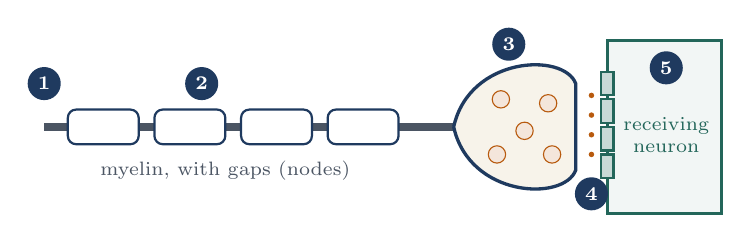
\begin{tikzpicture}[x=1cm,y=1cm]
    % axon with myelin
    \draw[kgrey,line width=3pt] (0,0) -- (5.2,0);
    \foreach \x in {0.3,1.4,2.5,3.6}{\draw[myel] (\x,-0.22) rectangle (\x+0.9,0.22);}
    \node[font=\scriptsize,text=kgrey] at (2.3,-0.55) {myelin, with gaps (nodes)};
    % terminal
    \draw[kprimary,very thick,fill=kpale] (5.2,0.0) .. controls (5.4,0.9) and (6.6,0.95) .. (6.75,0.55) -- (6.75,-0.55) .. controls (6.6,-0.95) and (5.4,-0.9) .. (5.2,0.0);
    \foreach \x/\y in {5.8/0.35,6.1/-0.05,5.75/-0.35,6.4/0.3,6.45/-0.35}{\node[ves] at (\x,\y) {};}
    % cleft and receiving cell
    \foreach \y in {-0.35,-0.1,0.15,0.4}{\node[tx] at (6.95,\y) {};}
    \draw[kgreen,very thick,fill=kgreen!6] (7.15,-1.1) -- (7.15,1.1) -- (8.6,1.1) -- (8.6,-1.1) -- cycle;
    \foreach \y in {-0.5,-0.15,0.2,0.55}{\node[rcp] at (7.15,\y) {};}
    \node[font=\scriptsize,text=kgreen,align=center] at (7.9,-0.1) {receiving\\neuron};
    % badges
    \node[badge] at (0.0,0.55) {1};
    \node[badge] at (2.0,0.55) {2};
    \node[badge] at (5.9,1.05) {3};
    \node[badge] at (6.95,-0.85) {4};
    \node[badge] at (7.9,0.75) {5};
  \end{tikzpicture}}
\newcommand{\relaylist}{%
  \begin{enumerate}\setlength{\itemsep}{3pt}
    \item \textbf{Along the axon:} each patch fires the next, like a fuse.
    \item \textbf{Myelin} makes the spike jump from gap to gap: much faster.
    \item \textbf{At the terminal:} \Ca\ rushes in; vesicles release transmitter.
    \item \textbf{Across the gap:} transmitter binds to \textbf{receptors}.
    \item \textbf{The receiving neuron} adds up its inputs and decides.
  \end{enumerate}}

% \saltpicture: bare versus myelinated conduction
\newcommand{\saltpicture}{%
  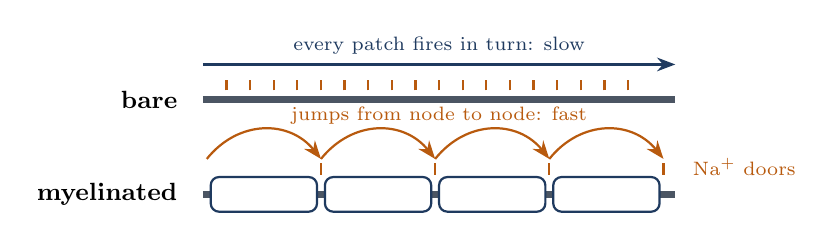
\begin{tikzpicture}[x=1cm,y=1cm]
    \node[font=\small\bfseries,anchor=east] at (-0.2,1.2) {bare};
    \draw[kgrey,line width=2.5pt] (0,1.2) -- (6,1.2);
    \foreach \x in {0.3,0.6,...,5.7}{\draw[cNa,thick] (\x,1.32) -- (\x,1.45);}
    \draw[-{Stealth},thick,kprimary] (0,1.65) -- (6,1.65) node[midway,above,font=\scriptsize]{every patch fires in turn: slow};
    \node[font=\small\bfseries,anchor=east] at (-0.2,0) {myelinated};
    \draw[kgrey,line width=2.5pt] (0,0) -- (6,0);
    \foreach \x in {0.1,1.55,3.0,4.45}{\draw[myel] (\x,-0.22) rectangle (\x+1.35,0.22);}
    \foreach \x in {1.5,2.95,4.4,5.85}{\draw[cNa,thick] (\x,0.25) -- (\x,0.4);}
    \foreach \a/\b in {0.05/1.5,1.5/2.95,2.95/4.4,4.4/5.85}{\draw[-{Stealth},thick,kaccent] (\a,0.45) .. controls (\a+0.4,0.95) and (\b-0.4,0.95) .. (\b,0.45);}
    \node[font=\scriptsize,text=kaccent] at (3,1.0) {jumps from node to node: fast};
    \node[font=\scriptsize,text=cNa,anchor=west] at (6.1,0.35) {Na$^{+}$ doors};
  \end{tikzpicture}}

% \synapsesteps: the six steps of a chemical synapse
\newcommand{\synapsesteps}{%
  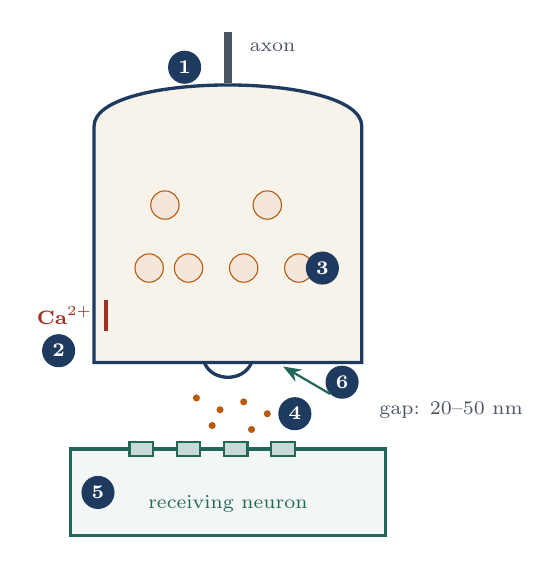
\begin{tikzpicture}[x=1cm,y=1cm]
    \draw[kprimary,very thick,fill=kpale] (0,0.2) -- (0,3.2) .. controls (0,3.9) and (3.4,3.9) .. (3.4,3.2) -- (3.4,0.2) -- cycle;
    \draw[kgrey,line width=3pt] (1.7,3.75) -- (1.7,4.4);
    \node[font=\scriptsize,text=kgrey,anchor=west] at (1.85,4.2) {axon};
    \foreach \x/\y in {0.7,1.2,1.9,2.6}{\node[ves,minimum size=0.36cm] at (\x,1.4) {};}
    \foreach \x in {0.9,2.2}{\node[ves,minimum size=0.36cm] at (\x,2.2) {};}
    \draw[cCa,very thick] (0.15,0.6) -- (0.15,1.0); \node[font=\scriptsize\bfseries,text=cCa,anchor=east] at (0.1,0.8) {Ca$^{2+}$};
    \draw[kprimary,very thick] (1.4,0.2) .. controls (1.5,-0.05) and (1.9,-0.05) .. (2.0,0.2);
    \foreach \x/\y in {1.3/-0.25,1.6/-0.4,1.9/-0.3,2.2/-0.45,1.5/-0.6,2.0/-0.65}{\node[tx,minimum size=0.09cm] at (\x,\y) {};}
    \draw[kgreen,very thick,fill=kgreen!6] (-0.3,-0.9) -- (3.7,-0.9) -- (3.7,-2.0) -- (-0.3,-2.0) -- cycle;
    \foreach \x in {0.6,1.2,1.8,2.4}{\node[rcp,minimum width=0.3cm,minimum height=0.18cm] at (\x,-0.9) {};}
    \node[font=\scriptsize,text=kgreen] at (1.7,-1.6) {receiving neuron};
    \node[font=\scriptsize,text=kgrey,anchor=west] at (3.5,-0.4) {gap: 20--50 nm};
    \node[badge] at (1.15,3.95) {1};
    \node[badge] at (-0.45,0.35) {2};
    \node[badge] at (2.9,1.4) {3};
    \node[badge] at (2.55,-0.45) {4};
    \node[badge] at (0.05,-1.45) {5};
    \node[badge] at (3.15,-0.05) {6};
    \draw[-{Stealth},kgreen,thick] (3.0,-0.2) -- (2.4,0.15);
  \end{tikzpicture}}
\newcommand{\synapselist}{%
  \begin{enumerate}\setlength{\itemsep}{2pt}
    \item A spike arrives at the terminal.
    \item \Ca\ doors open; \Ca\ rushes in.
    \item Vesicles fuse and release transmitter.
    \item Transmitter crosses the gap and binds to receptors.
    \item Receptor channels open: an \textbf{EPSP} or \textbf{IPSP}.
    \item Transmitter is cleared: reuptake or an enzyme.
  \end{enumerate}}
% ---- the Relay Lab link: change here if the page moves; the QR codes update themselves ----
\newcommand{\lablink}{https://rakesh-sengupta.github.io/neural-signalling-labs/labs/relay-lab/}
\newcommand{\lablinkshown}{rakesh-sengupta.github.io/\\neural-signalling-labs/\\labs/relay-lab}

% ---- Relay Lab passwords: one per part, shown only on that part's lab slide.
%      They must match PASSWORDS at the top of the lab's script (index.html). Case is ignored. ----
\newcommand{\pwone}{cheetah}
\newcommand{\pwtwo}{chorus}
\newcommand{\pwthree}{keyring}
\newcommand{\labpw}[1]{\ifcase#1\or\pwone\or\pwtwo\or\pwthree\fi}

% ---- "so far" recap tiles: colour, title, text, x position ----
\newcommand{\recaptile}[4]{\node[draw=#1,fill=#1!8,rounded corners=4pt,text width=4.1cm,minimum height=2.6cm,align=center,font=\normalsize] at (#4,0) {{\large\bfseries\color{#1}#2}\\[4pt]#3};}

% ---- lab activity slide: part, title, minutes, booklet page, steps, done-when ----
\newcommand{\labframe}[6]{%
\begin{frame}{Relay Lab, Part #1: #2}{\tLab}
  \actinfo{#3}{alone or in pairs}{laptop or phone, booklet page #4}
  \begin{columns}[T]
    \begin{column}{0.68\textwidth}
      \begin{enumerate}\setlength{\itemsep}{2pt}
        \item Type the \textbf{password} (right) and press \textbf{Unlock}.
        #5
      \end{enumerate}
      \vspace{0.3em}
      \begin{donebox}#6\end{donebox}
    \end{column}
    \begin{column}{0.29\textwidth}
      \centering
      {\setlength{\fboxsep}{5pt}\fcolorbox{kaccent}{kaccent!10}{\parbox{0.9\linewidth}{\centering
        {\scriptsize\bfseries\color{kgrey}PASSWORD}\\[1pt]{\Large\bfseries\color{kprimary}\labpw{#1}}}}}\\[4pt]
      \qrcode[height=1.9cm]{\lablink}\\[2pt]
      {\scriptsize\lablinkshown}
    \end{column}
  \end{columns}
\end{frame}}

\title{The Relay}
\subtitle{How signals travel along axons, cross synapses, and act on receptors}
\author{Rakesh Sengupta}
\institute{School of Interwoven Arts and Sciences, Krea University}
\date{Introduction to Neuroscience \,$\cdot$\, Sessions \sessnum\ (combined) \,$\cdot$\, Reading: Bear et al., Ch.~4 (end), 5 and 6}

\begin{document}

% =====================================================================
\begin{frame}[plain]
  \begin{tikzpicture}[remember picture,overlay]
    \fill[kprimary] (current page.north west) rectangle ([yshift=-1.3cm]current page.north east);
    \fill[kaccent] ([yshift=-1.3cm]current page.north west) rectangle ([yshift=-1.42cm]current page.north east);
  \end{tikzpicture}
  \vspace{1.2cm}
  \titlepage
\end{frame}

% =====================================================================
\begin{frame}{Plan for today}{\tPlan}
  \renewcommand{\arraystretch}{1.3}
  \begin{tabular}{@{}>{\raggedright\arraybackslash\bfseries}p{3.3cm}>{\raggedright\arraybackslash}p{8.0cm}r@{}}
    \toprule
    Part & What we do & Time\\
    \midrule
    Opening & From one spike to the next neuron; open Relay Lab & 7 min\\
    1 Along the axon & How a spike travels; myelin; MS (Lab Part 1) & 25 min\\
    2 Across the gap & Sparks or soups? The chemical synapse; adding up (Lab Part 2) & 28 min\\
    3 Keys and locks & Transmitters, receptors, drugs (Lab Part 3) & 22 min\\
    Wrap-up & Today on one page, again; exit ticket & 8 min\\
    \bottomrule
  \end{tabular}
  \vspace{0.6em}

  \small\textbf{You need:} a laptop or phone (or a partner with one), the booklet, a pen. \textbf{Lost?} Booklet page 2 has today on one page.\\[2pt]
  \textbf{Next class: Quiz 2} (Sessions 7--12).
  \note{This combined session covers three outline sessions (axonal conduction, synaptic transmission, transmitter systems). It is dense: the "So far" slides are the planned pauses. If time is short, skip the slides marked (optional) in the notes; everything skipped is in the booklet.}
\end{frame}

% =====================================================================
\begin{frame}{How these slides work}{\tPlan}
  \glance{The bold line at the top of each slide is the one thing to remember.}
  \begin{columns}[T]
    \begin{column}{0.5\textwidth}
      Labels at the top right:\\[5pt]
      \tIdea\ \ one idea \quad \tStudy\ \ a real finding\\[4pt]
      \tThink\ \ a question for you\\[4pt]
      \tLab\ \ do this part of the lab \quad \tAns\ \ answers
    \end{column}
    \begin{column}{0.47\textwidth}
      Colours stay the same as before:\\[5pt]
      \Na\ sodium \quad \K\ potassium\\[4pt]
      \Cl\ chloride \quad \Ca\ calcium\\[8pt]
      You can write instead of speaking, or pass.
    \end{column}
  \end{columns}
\end{frame}

% =====================================================================
\renewcommand{\sectionsub}{From one spike to the next neuron}
\section{Opening}

\begin{frame}{Warm-up}{\tThink}
  \begin{askbox}
    You touch a hot pan. The message must travel about a metre up your arm, then pass from one neuron to the next, several times.\\[6pt]
    \textbf{Where would you guess the time is lost: on the long trip along the wires, or at the junctions between them?} Write a guess on booklet page 1.
  \end{askbox}
  \note{Link to the interlude (Donders): most of a reaction is processing, not travel. Today shows both halves: travel along axons, and the junctions.}
\end{frame}

% =====================================================================
\begin{frame}{Today on one page}{\tIdea}
  \glance{One relay: along the axon, across the gap, into the next neuron.}
  \begin{columns}[c]
    \begin{column}{0.56\textwidth}
      \centering\resizebox{\linewidth}{!}{\relaypicture}
    \end{column}
    \begin{column}{0.42\textwidth}
      \small\relaylist
    \end{column}
  \end{columns}
  \note{Show it, do not explain it yet. It returns at the end. The same picture is on booklet page 2.}
\end{frame}

% =====================================================================
\begin{frame}{Open Relay Lab now}{\tLab}
  \glance{Keep the lab open beside the slides. Each lab slide tells you which part.}
  \begin{columns}[c]
    \begin{column}{0.6\textwidth}
      \begin{itemize}\setlength{\itemsep}{6pt}
        \item Three short parts: \textbf{the race}, \textbf{adding up}, \textbf{keys and locks}. About 8 minutes each.
        \item Works on a laptop or a phone. Nobody sees your answers.
        \item \textbf{Nothing is saved or sent.}
        \item Press \textbf{Continue}. Each part is \textbf{locked}: its password appears on its lab slide. No rush.
      \end{itemize}
    \end{column}
    \begin{column}{0.37\textwidth}
      \centering
      \qrcode[height=3.1cm]{\lablink}\\[4pt]
      {\footnotesize\lablinkshown}
    \end{column}
  \end{columns}
  \note{No device? Pair up: one person drives, the other reads the steps aloud and writes the numbers.}
\end{frame}

% =====================================================================
\renewcommand{\sectionsub}{How a spike travels; myelin; multiple sclerosis}
\section{1 Along the axon}

\begin{frame}{A spike travels like a burning fuse}{\tIdea}
  \glance{Each patch of axon fires the next patch, so the spike arrives full size.}
  \begin{itemize}\setlength{\itemsep}{8pt}
    \item \Na\ rushing in at one patch spreads a little way inside the axon, pushing the next patch to threshold.
    \item The patch behind is refractory (Session 9), so the spike cannot turn back.
    \item A typical speed is about \textbf{10 m/s}, so one 2 ms spike is spread over about \textbf{2 cm} of axon \src{Bear et al., Ch.~4}.
  \end{itemize}
  \note{Bear compares conduction to a lit fuse: the heat at one point ignites the next. Unlike a fuse, the axon recovers and can fire again. Spikes started artificially at the far end can travel backwards (antidromic), but in the body they travel from cell body to terminal.}
\end{frame}

% =====================================================================
\begin{frame}{What sets the speed? Thickness}{\tIdea}
  \glance{A wider axon lets the current spread farther ahead, so it is faster.}
  \begin{itemize}\setlength{\itemsep}{8pt}
    \item Current ahead of the spike has two paths: \textbf{along} the inside of the axon, or \textbf{out} through the membrane. Bear compares this to water in a leaky garden hose.
    \item A wide axon carries more current along it, so the next patch reaches threshold sooner.
    \item The squid's escape axon is up to \textbf{1 mm} wide, so wide that it was first mistaken for a blood vessel \src{Bear et al., Ch.~4}.
  \end{itemize}
  \note{This is the squid giant axon from the interlude and Session 9. Small axons also need more depolarisation to fire and are blocked sooner by local anaesthetics, which is why the dentist's lidocaine silences thin pain fibres first (Bear, Box 4.4).}
\end{frame}

% =====================================================================
\begin{frame}{Myelin: a faster trick than thickness}{\tIdea}
  \glance{Myelin insulates the axon, so the spike jumps from gap to gap.}
  \begin{columns}[c]
    \begin{column}{0.58\textwidth}
      \centering\resizebox{\linewidth}{!}{\saltpicture}
    \end{column}
    \begin{column}{0.4\textwidth}
      \begin{itemize}\setlength{\itemsep}{6pt}
        \item Glia wrap the axon in layers of membrane: \textbf{myelin} (Session 6).
        \item Gaps called \textbf{nodes of Ranvier}, 0.2--2 mm apart, hold the \Na\ doors.
        \item The spike leaps node to node: \textbf{saltatory} conduction (Latin \emph{saltare}, to leap).
      \end{itemize}
    \end{column}
  \end{columns}
  \src{Bear et al., Ch.~4}
  \note{Bear's image: unmyelinated conduction is walking heel-to-toe along a pavement; myelinated conduction is skipping. If all your axons were as thick as a squid's, your head would not fit through a door. Myelin is made by oligodendrocytes in the brain and spinal cord, and Schwann cells in the body.}
\end{frame}

% =====================================================================
\begin{frame}{How fast is fast?}{\tIdea}
  \glance{From walking pace to a racing car: about 1 to 120 m/s.}
  \renewcommand{\arraystretch}{1.4}
  \begin{tabular}{@{}l l l@{}}
    \toprule
    Axon & Example & Speed\\
    \midrule
    thin, bare (about 1 \textmu m) & slow, aching pain & about \textbf{1 m/s}\\
    squid giant axon (0.5--1 mm, bare) & squid escape jet & about \textbf{20 m/s}\\
    thick, myelinated (13--20 \textmu m) & muscle sense, movement & \textbf{80--120 m/s}\\
    \bottomrule
  \end{tabular}
  \vspace{0.6em}

  \raggedright
  A myelinated axon a fiftieth of the squid's width is several times faster. That is how a brain fits billions of fast axons into a skull.
  \src{Erlanger--Gasser fibre classes; Purves et al., \emph{Neuroscience}}
  \note{Rule of thumb for mammalian myelinated axons: about 6 m/s per micrometre of diameter (Hursh, 1939). Link to Session 5: the sharp first pain and the dull later ache travel on different fibres.}
\end{frame}

% =====================================================================
\begin{frame}{When myelin is lost: multiple sclerosis}{\tStudy}
  \glance{In MS, damaged myelin slows or blocks the spike.}
  \begin{itemize}\setlength{\itemsep}{7pt}
    \item MS attacks myelin in the brain, spinal cord and optic nerves, at many sites; it often comes and goes over years.
    \item Symptoms: weakness, poor coordination, blurred vision, slurred speech.
    \item A test: show a checkerboard, and time the response over the visual cortex. In MS it arrives late \src{Bear et al., Box 4.5}.
  \end{itemize}
  \vspace{0.2em}
  \begin{factbox}
    In Guillain--Barr\'e syndrome, the immune system attacks myelin in the nerves of the body instead, slowing signals to the muscles.
  \end{factbox}
  \note{"Sclerosis" is Greek for hardening: the scarred patches. The checkerboard test measures visual evoked potentials. Treat this sensitively: some students may know someone with MS.}
\end{frame}

% =====================================================================
\labframe{1}{the race}{8 min}{4}%
  {\item Choose an axon and press \textbf{Send a spike}. It races 10 cm between two electrodes.
   \item Race four: \textbf{1 \textmu m bare}; \textbf{12 \textmu m myelinated}; the \textbf{squid giant axon}; \textbf{12 \textmu m myelinated with damaged myelin}.
   \item Read each speed from the table; type it in and press \textbf{Check}.}%
  {Four speeds are in the booklet and you answered the two questions.}

% =====================================================================
\begin{frame}{Relay Lab, Part 1: answers}{\tAns}
  \glance{Myelin beats size. Damaged myelin slows the spike about sevenfold.}
  \renewcommand{\arraystretch}{1.35}
  \begin{tabular}{@{}l r r@{}}
    \toprule
    Axon & Time for 10 cm & Speed\\
    \midrule
    1 \textmu m, bare & 100 ms & \textbf{1 m/s}\\
    12 \textmu m, myelinated & 1.4 ms & \textbf{72 m/s}\\
    squid giant axon (500 \textmu m, bare) & 4.5 ms & \textbf{22 m/s}\\
    12 \textmu m, damaged myelin patch & 9.6 ms & \textbf{10 m/s}\\
    \bottomrule
  \end{tabular}
  \vspace{0.5em}

  \raggedright
  At 1 m/s, a pain message takes about a second to travel a metre; at 72 m/s, about 14 ms.
  \note{The lab's speeds come from rules of thumb fitted to real nerves (6 m/s per micrometre myelinated; square root of diameter for bare axons), not from a simulation. The damaged patch covers 3 of the 10 cm.}
\end{frame}

% =====================================================================
\begin{frame}{So far}{\tIdea}
  \glance{Spikes travel like a fuse; thickness and myelin make them fast.}
  \centering
  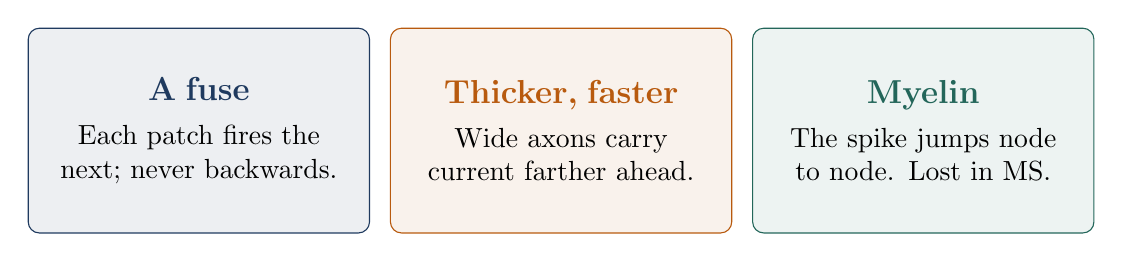
\begin{tikzpicture}
    \recaptile{kprimary}{A fuse}{Each patch fires the next; never backwards.}{0}
    \recaptile{kaccent}{Thicker, faster}{Wide axons carry current farther ahead.}{4.6}
    \recaptile{kgreen}{Myelin}{The spike jumps node to node. Lost in MS.}{9.2}
  \end{tikzpicture}
  \par\vspace{0.6em}
  {\small Next: the spike reaches the end of the axon. How does it get to the next neuron?}
\end{frame}

% =====================================================================
\renewcommand{\sectionsub}{Sparks or soups? The chemical synapse; adding up}
\section{2 Across the gap}

\begin{frame}{The war of the soups and the sparks}{\tStudy}
  \glance{For decades, scientists argued: is the message across a synapse electrical or chemical?}
  \begin{itemize}\setlength{\itemsep}{6pt}
    \item \textbf{Sparks:} physiologists led by John Eccles: only electricity is fast enough.
    \item \textbf{Soups:} Henry Dale and Otto Loewi (the dream, from the interlude): chemicals.
    \item Karl Popper urged Eccles to make his theory testable enough to be \textbf{proved wrong}. In 1951, Eccles's own experiments did \src{Valenstein, 2005}.
  \end{itemize}
  \vspace{0.2em}
  \begin{askbox}
    Eccles switched sides, and won a Nobel Prize in 1963. Is changing your mind a weakness or a strength in science?
  \end{askbox}
  \note{Popper's falsificationism: good theories risk being shown false. Historians note that Popper's influence was more on how Eccles framed his work than on his experiments (Borck, 2017). The answer was "mostly soups": well under 1 percent of synapses turned out to be electrical.}
\end{frame}

% =====================================================================
\begin{frame}{Two kinds of synapse}{\tIdea}
  \glance{Electrical synapses pass current directly. Chemical synapses use a messenger.}
  \begin{columns}[T]
    \begin{column}{0.48\textwidth}
      \begin{factbox}[title={Electrical (gap junction)}]
        Cells only about \textbf{3 nm} apart, joined by protein pores. Current flows straight through: very fast, usually both ways. Common where neurons must fire together.
      \end{factbox}
    \end{column}
    \begin{column}{0.48\textwidth}
      \begin{factbox}[colframe=kgreen,colback=kgreen!5,title={Chemical}]
        A gap of \textbf{20--50 nm}. The sender releases a \textbf{neurotransmitter}; the receiver has \textbf{receptors}. One-way, slightly slower, but adjustable. Most brain synapses.
      \end{factbox}
    \end{column}
  \end{columns}
  \src{Bear et al., Ch.~5}
  \note{Charles Sherrington named the synapse in 1897. Electrical synapses help groups of neurons, for example in the brain stem, fire in synchrony.}
\end{frame}

% =====================================================================
\begin{frame}{A chemical synapse in six steps}{\tIdea}
  \glance{Electrical signal $\rightarrow$ chemical $\rightarrow$ electrical again, in about a millisecond.}
  \begin{columns}[c]
    \begin{column}{0.48\textwidth}
      \centering\resizebox{!}{4.7cm}{\synapsesteps}
    \end{column}
    \begin{column}{0.5\textwidth}
      \small\synapselist
      \src{Bear et al., Ch.~5}
    \end{column}
  \end{columns}
  \note{Vesicles are about 50 nm across; release can follow calcium entry within 0.2 ms. Release of the vesicle's contents is exocytosis; the vesicle membrane is later recovered and refilled. Botulinum toxin (Botox) blocks step 3 at muscle synapses; black widow venom forces it (Bear, Box 5.5). The order of the six steps is the first task in Lab Part 2.}
\end{frame}

% =====================================================================
\begin{frame}{Messages come in packets}{\tStudy}
  \glance{Transmitter is released in whole vesicles, called quanta.}
  \begin{itemize}\setlength{\itemsep}{8pt}
    \item Bernard Katz found that responses come in steps, each the size of one vesicle's contents: a \textbf{quantum} of several thousand molecules.
    \item At a muscle, one spike releases about \textbf{200 vesicles}: a response of 40 mV or more, so the muscle always fires.
    \item At a typical brain synapse, often \textbf{one vesicle}: a response of a few tenths of a millivolt \src{Bear et al., Ch.~5}.
  \end{itemize}
  \note{Katz shared the 1970 Nobel Prize. The contrast sets up summation: a brain neuron needs many inputs at once.}
\end{frame}

% =====================================================================
\begin{frame}{Pushes up and pushes down}{\tIdea}
  \glance{Excitatory inputs push towards threshold (EPSP). Inhibitory inputs pull away (IPSP).}
  \begin{columns}[c]
    \begin{column}{0.48\textwidth}
      \centering
      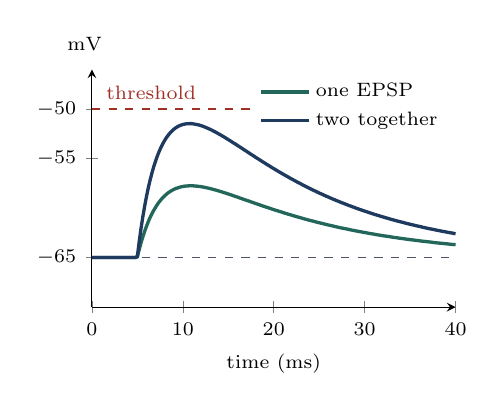
\begin{tikzpicture}
        \begin{axis}[lifstyle, width=6.2cm, height=4.6cm, ymin=-70, ymax=-46, ytick={-65,-55,-50}, yticklabels={$-65$,$-55$,$-50$}, legend style={font=\scriptsize, draw=none, fill=white, at={(0.99,0.99)}, anchor=north east}, legend cell align=left]
          \addplot[kgrey, dashed, domain=0:40, samples=2] {-65};
          \addplot[kred, dashed, domain=0:40, samples=2] {-50};
          \addplot[kgreen, very thick] coordinates {\lifA};
          \addplot[kprimary, very thick] coordinates {\lifAB};
          \legend{,,one EPSP,two together}
          \node[font=\scriptsize,text=kred,anchor=south west] at (axis cs:0.5,-50) {threshold};

        \end{axis}
      \end{tikzpicture}
    \end{column}
    \begin{column}{0.5\textwidth}
      \begin{itemize}\setlength{\itemsep}{6pt}
        \item \textbf{Glutamate} usually excites: channels let positive ions in.
        \item \textbf{GABA} and \textbf{glycine} usually inhibit: \Cl\ channels hold the voltage near rest.
        \item One input is rarely enough. The neuron must \textbf{add up} its inputs.
      \end{itemize}
    \end{column}
  \end{columns}
  \note{Traces come from the Relay Lab Part 2 model neuron. EPSP: excitatory postsynaptic potential; IPSP: inhibitory. In the model each EPSP is about 7 mV; real ones are usually far smaller.}
\end{frame}

% =====================================================================
\begin{frame}{Adding up: space and time}{\tIdea}
  \glance{Inputs add up if they arrive together (spatial) or close in time (temporal).}
  \begin{columns}[c]
    \begin{column}{0.48\textwidth}
      \centering
      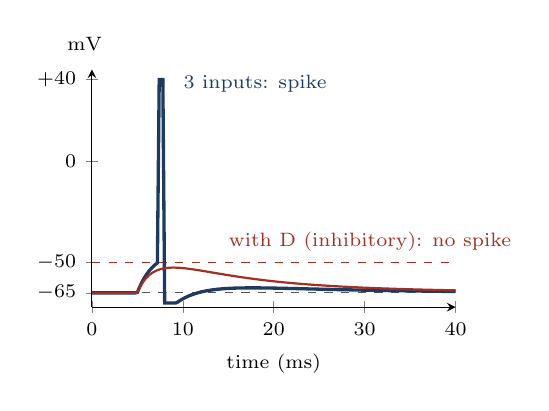
\begin{tikzpicture}
        \begin{axis}[lifstyle, width=6.2cm, height=4.6cm, xmax=40]
          \addplot[kgrey, dashed, domain=0:40, samples=2] {-65};
          \addplot[kred, dashed, domain=0:40, samples=2] {-50};
          \addplot[kprimary, very thick] coordinates {\lifABC};
          \addplot[kred, thick] coordinates {\lifABCD};
          \node[font=\scriptsize,text=kprimary,anchor=west] at (axis cs:9,38) {3 inputs: spike};
          \node[font=\scriptsize,text=kred,anchor=west] at (axis cs:14,-40) {with D (inhibitory): no spike};
        \end{axis}
      \end{tikzpicture}
    \end{column}
    \begin{column}{0.5\textwidth}
      \begin{itemize}\setlength{\itemsep}{6pt}
        \item \textbf{Spatial} summation: many synapses at once.
        \item \textbf{Temporal} summation: one synapse, firing again within about 1--15 ms \src{Bear et al., Ch.~5}.
        \item An inhibitory input can veto the lot.
      \end{itemize}
    \end{column}
  \end{columns}
  \note{Inhibitory synapses near the cell body are especially powerful: shunting inhibition, like cutting a hole in the hose ahead of the spike-initiation zone. Bear's Box 5.6: startle disease and strychnine, a glycine antagonist, show what happens when inhibition fails.}
\end{frame}

% =====================================================================
\labframe{2}{adding up}{8 min}{5}%
  {\item Put the six steps of a chemical synapse in order.
   \item Fire A alone, then A + B, then A + B + C. Then add D.
   \item Fire A three times; find the longest gap that still makes a spike.}%
  {The steps are in order, three numbers are checked, and two questions are answered.}

% =====================================================================
\begin{frame}{Relay Lab, Part 2: answers}{\tAns}
  \glance{Three inputs together, or one input three times within 7 ms. Inhibition vetoes.}
  \renewcommand{\arraystretch}{1.35}
  \begin{tabular}{@{}l l@{}}
    \toprule
    Rise from A alone & about \textbf{7 mV} (threshold is 15 mV above rest)\\
    A + B together & about 13.5 mV: \textbf{still no spike}\\
    Inputs needed together & \textbf{3}\\
    A three times & spike up to a \textbf{7 ms} gap; none at 8 ms\\
    A + B + C + D & \textbf{no spike}: inhibition\\
    \bottomrule
  \end{tabular}
  \vspace{0.5em}

  \raggedright
  A brain neuron is a decision-maker, not a relay: it weighs thousands of inputs. A muscle synapse, by contrast, must work every time.
  \note{The lab uses a leaky integrate-and-fire neuron with a 15 ms membrane time constant, chosen to show the 1-15 ms summation window. Real cortical neurons receive thousands of synapses with much smaller EPSPs.}
\end{frame}

% =====================================================================
\begin{frame}{So far}{\tIdea}
  \glance{At most synapses, a chemical carries the message, and the receiving neuron adds it up.}
  \centering
  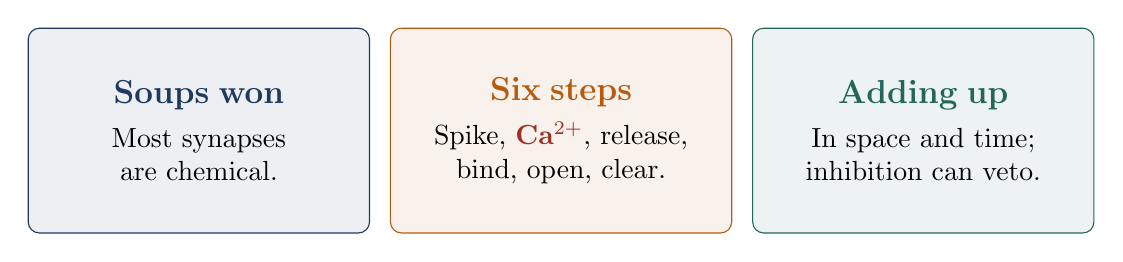
\begin{tikzpicture}
    \recaptile{kprimary}{Soups won}{Most synapses are chemical.}{0}
    \recaptile{kaccent}{Six steps}{Spike, \Ca, release, bind, open, clear.}{4.6}
    \recaptile{kgreen}{Adding up}{In space and time; inhibition can veto.}{9.2}
  \end{tikzpicture}
  \par\vspace{0.6em}
  {\small Next: which chemicals, which receptors, and how drugs get in on the act.}
\end{frame}

% =====================================================================
\renewcommand{\sectionsub}{Transmitters, receptors, drugs}
\section{3 Keys and locks}

\begin{frame}{Three families of transmitter}{\tIdea}
  \glance{Neurotransmitters are amino acids, amines, or peptides.}
  \renewcommand{\arraystretch}{1.4}
  \begin{tabular}{@{}l >{\raggedright\arraybackslash}p{5.0cm} >{\raggedright\arraybackslash}p{4.6cm}@{}}
    \toprule
    Family & Examples & Typical job\\
    \midrule
    Amino acids & \textbf{glutamate}, \textbf{GABA}, glycine & fast excitation or inhibition\\
    Amines & \textbf{ACh}, dopamine, noradrenaline, serotonin & muscles; mood, attention, movement\\
    Peptides & enkephalins (the brain's own opioids) & slow, long-lasting, e.g.\ pain\\
    \bottomrule
  \end{tabular}
  \vspace{0.4em}

  \src{Bear et al., Ch.~6}
  \note{Dale's principle: a neuron uses the same transmitter at all its terminals, hence names such as cholinergic, glutamatergic, GABAergic. Many peptide neurons break it by releasing a peptide alongside another transmitter.}
\end{frame}

% =====================================================================
\begin{frame}{Two kinds of lock}{\tIdea}
  \glance{Ion-channel receptors are fast. G-protein receptors are slow, but amplify.}
  \begin{columns}[c]
    \begin{column}{0.5\textwidth}
      \centering
      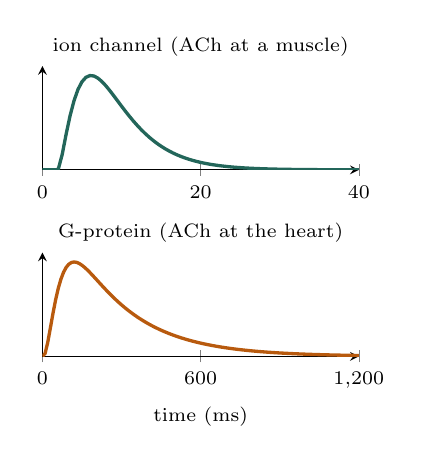
\begin{tikzpicture}
        \begin{axis}[name=a1, axis lines=left, width=5.6cm, height=2.9cm, xmin=0, xmax=40, ymin=0, ymax=110, ytick=\empty, xtick={0,20,40}, tick label style={font=\scriptsize}, title={\scriptsize ion channel (ACh at a muscle)}, title style={yshift=-6pt}]
          \addplot[kgreen, very thick] coordinates {\recnic};
        \end{axis}
        \begin{axis}[at={(a1.south west)}, anchor=north west, yshift=-1.05cm, axis lines=left, width=5.6cm, height=2.9cm, xmin=0, xmax=1200, ymin=0, ymax=110, ytick=\empty, xtick={0,600,1200}, tick label style={font=\scriptsize}, xlabel={time (ms)}, label style={font=\scriptsize}, title={\scriptsize G-protein (ACh at the heart)}, title style={yshift=-6pt}]
          \addplot[kaccent, very thick] coordinates {\recmus};
        \end{axis}
      \end{tikzpicture}
    \end{column}
    \begin{column}{0.48\textwidth}
      \begin{itemize}\setlength{\itemsep}{6pt}
        \item \textbf{Ion channel:} the receptor \emph{is} the door. Opens within a millisecond.
        \item \textbf{G-protein-coupled:} the receptor switches on a chain of molecules inside the cell. Slower, longer.
        \item One receptor can switch on 10--20 G-proteins: \textbf{amplification} \src{Bear et al., Ch.~6}.
      \end{itemize}
    \end{column}
  \end{columns}
  \note{Note the time axes: 40 ms versus 1200 ms. Traces are from the Relay Lab Part 3 model. Older names: ionotropic and metabotropic receptors. Long-lasting chemical changes triggered by cascades may underlie memory (Session 17).}
\end{frame}

% =====================================================================
\begin{frame}{One key, many locks}{\tIdea}
  \glance{The same transmitter can do opposite things, depending on the receptor.}
  \begin{itemize}\setlength{\itemsep}{8pt}
    \item ACh at a skeletal muscle: \textbf{nicotinic} receptors (ion channels). The muscle contracts.
    \item ACh at the heart: \textbf{muscarinic} receptors (G-protein). The heart slows.
    \item This is \textbf{divergence}: every known transmitter acts on several receptor types \src{Bear et al., Ch.~6}.
  \end{itemize}
  \vspace{0.2em}
  \begin{factbox}
    So ``dopamine is the pleasure chemical'' is too simple: what a transmitter does depends on where it lands.
  \end{factbox}
  \note{The receptor names come from the drugs that activate them: nicotine (tobacco) and muscarine (a mushroom toxin). Convergence is the reverse: several transmitters acting on one cell through the same internal pathway.}
\end{frame}

% =====================================================================
\begin{frame}{How drugs act at a synapse}{\tIdea}
  \glance{Drugs copy the key, block the lock, or keep the key in the lock longer.}
  \renewcommand{\arraystretch}{1.35}
  \begin{tabular}{@{}l >{\raggedright\arraybackslash}p{4.6cm} >{\raggedright\arraybackslash}p{5.0cm}@{}}
    \toprule
    Kind of drug & What it does & Examples\\
    \midrule
    \textbf{Agonist} & copies the transmitter & nicotine (ACh receptors)\\
    \textbf{Antagonist} & blocks the receptor & curare (ACh); caffeine (adenosine)\\
    \textbf{Reuptake blocker} & keeps transmitter in the gap & fluoxetine/Prozac (serotonin)\\
    \textbf{Enzyme blocker} & stops its breakdown & AChE inhibitors\\
    \bottomrule
  \end{tabular}
  \vspace{0.3em}

  \src{Bear et al., Ch.~5 and Table 6.1}
  \note{Curare: an arrow-tip poison that paralyses prey. Some Alzheimer's medicines are mild AChE inhibitors; nerve agents are extreme ones. Strychnine is a glycine antagonist (Box 5.6). Keep the discussion at the level of mechanism.}
\end{frame}

% =====================================================================
\labframe{3}{keys and locks}{8 min}{6}%
  {\item Pick a synapse; press \textbf{Release transmitter} with no drug.
   \item Try the agonist, the antagonist and the clearance blocker. Watch both panels.
   \item Compare the muscle (ion channel) with a G-protein synapse.}%
  {You tried all three drugs on two synapses and filled in the booklet table.}

% =====================================================================
\begin{frame}{Relay Lab, Part 3: answers}{\tAns}
  \glance{Agonist: response even without release. Antagonist: tiny. Blocker: bigger, longer.}
  \renewcommand{\arraystretch}{1.3}
  \begin{tabular}{@{}l c c@{}}
    \toprule
    Drug & Muscle (ion channel) & Serotonin (G-protein)\\
    \midrule
    none & 100, about 8 ms & 100, about 320 ms\\
    agonist (nicotine) & already on; peak 150 & already on; peak 160\\
    antagonist (curare, caffeine) & 15 & 15\\
    clearance blocker (Prozac) & 210, about 22 ms & 290, about 590 ms\\
    \bottomrule
  \end{tabular}
  \vspace{0.5em}

  \raggedright
  The ion-channel response is over in milliseconds; the G-protein response lasts hundreds. Same rules, different timescales.
  \note{Arbitrary units, scaled so that no drug = 100; durations are time above half the peak. The model is simplified: the directions of the effects are what matter.}
\end{frame}

% =====================================================================
\begin{frame}{Finding the brain's own morphine}{\tStudy}
  \glance{Drugs revealed receptors, and receptors revealed the brain's own chemicals.}
  \begin{enumerate}\setlength{\itemsep}{6pt}
    \item In the 1970s, Solomon Snyder and his student Candace Pert labelled opiate drugs with radioactivity.
    \item The drugs stuck to specific sites on some neurons: \textbf{opiate receptors}.
    \item Why would the brain have receptors for a poppy drug? The search found the brain's own opioids, the \textbf{enkephalins} and endorphins \src{Bear et al., Ch.~6 and Box 6.1}.
  \end{enumerate}
  \vspace{0.2em}
  \begin{askbox}
    If the brain makes its own ``morphine'', what might it be for? (Hint: think of injuries during escape.)
  \end{askbox}
  \note{Endorphin: endogenous morphine. Possible answers: pain relief in emergencies, reward. A philosophical hint: drugs work only because they borrow the brain's own locks.}
\end{frame}

% =====================================================================
\begin{frame}{So far}{\tIdea}
  \glance{Which receptor a transmitter meets decides what it does; drugs hijack this.}
  \centering
  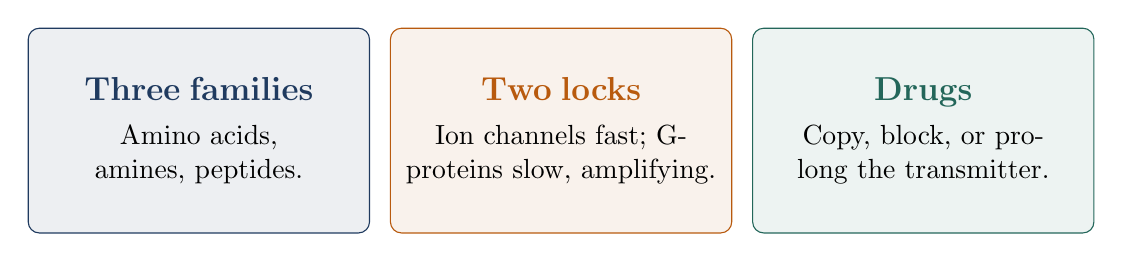
\begin{tikzpicture}
    \recaptile{kprimary}{Three families}{Amino acids, amines, peptides.}{0}
    \recaptile{kaccent}{Two locks}{Ion channels fast; G-proteins slow, amplifying.}{4.6}
    \recaptile{kgreen}{Drugs}{Copy, block, or prolong the transmitter.}{9.2}
  \end{tikzpicture}
\end{frame}

% =====================================================================
\renewcommand{\sectionsub}{Today on one page, exit ticket and next time}
\section{Wrap-up}

\begin{frame}{Today on one page, again}{\tThink}
  \glance{Can you explain each number to the person next to you?}
  \begin{columns}[c]
    \begin{column}{0.56\textwidth}
      \centering\resizebox{\linewidth}{!}{\relaypicture}
    \end{column}
    \begin{column}{0.42\textwidth}
      \small\relaylist
    \end{column}
  \end{columns}
  \note{Pairs take turns: one points at a number, the other explains it in one sentence. Two minutes. Back to the warm-up: most of the time in a reaction is lost at synapses and in adding up, not on the trip.}
\end{frame}

% =====================================================================
\begin{frame}{Three things to take away}{\tIdea}
  \begin{enumerate}\setlength{\itemsep}{9pt}
    \item A spike travels like a fuse. \textbf{Thick} and especially \textbf{myelinated} axons are fastest; MS damages myelin.
    \item At most synapses, \Ca\ triggers the release of a \textbf{chemical}; the receiving neuron \textbf{adds up} excitatory and inhibitory inputs.
    \item The \textbf{receptor} decides the response: fast ion channels or slow G-proteins. Drugs copy, block or prolong transmitters.
  \end{enumerate}
\end{frame}

% =====================================================================
\begin{frame}{Exit ticket and next time}{\tThink}
  \begin{columns}[T]
    \begin{column}{0.56\textwidth}
      \begin{askbox}[title={\bfseries Exit ticket: 3 minutes, booklet page 1}]
        \begin{enumerate}\setlength{\itemsep}{3pt}
          \item Why does myelin make a spike faster?
          \item What does \Ca\ do at the axon terminal?
          \item Name one agonist and one antagonist.
        \end{enumerate}
      \end{askbox}
    \end{column}
    \begin{column}{0.4\textwidth}
      \begin{factbox}[title={Next class}]
        \textbf{Quiz 2}, on Sessions 7--12: membranes, the resting and action potentials, conduction, synapses, transmitters.\\[4pt]
        \textbf{Revise with:} the ``today on one page'' sheets, and the three labs.
      \end{factbox}
    \end{column}
  \end{columns}
  \vspace{0.6em}
  \centering\large\color{kprimary}\textbf{Questions?}\quad{\small\color{kgrey}rakesh.sengupta@krea.edu.in}
\end{frame}

% =====================================================================
\begin{frame}{References}{\tRef}
  \fontsize{7.5}{8.8}\selectfont
  Bear, M.\,F., Connors, B.\,W., \& Paradiso, M.\,A.\ (2016). \emph{Neuroscience: Exploring the Brain} (4th ed.), Chapters 4 (conduction, Box 4.5), 5 and 6.\\[2pt]
  Borck, C.\ (2017). Soups and sparks revisited: John Eccles' path from the war on electrical transmission to mental sparks. \emph{Nuncius} 32, 286--329.\\[2pt]
  Brock, L.\,G., Coombs, J.\,S., \& Eccles, J.\,C.\ (1952). The recording of potentials from motoneurones with an intracellular electrode. \emph{J Physiol} 117, 431--460.\\[2pt]
  Hursh, J.\,B.\ (1939). Conduction velocity and diameter of nerve fibers. \emph{Am J Physiol} 127, 131--139.\\[2pt]
  Pert, C.\,B., \& Snyder, S.\,H.\ (1973). Opiate receptor: demonstration in nervous tissue. \emph{Science} 179, 1011--1014.\\[2pt]
  Purves, D., et al.\ \emph{Neuroscience} (Sinauer): fibre classes and conduction velocities.\\[2pt]
  Valenstein, E.\,S.\ (2005). \emph{The War of the Soups and the Sparks}. Columbia University Press.\\[4pt]
  Relay Lab: Part 1 uses published rules of thumb for conduction speed; Part 2 a leaky integrate-and-fire neuron; Part 3 a simplified receptor model. Built with jsPsych 7 (de Leeuw, 2015, \emph{Behav Res Methods} 47, 1--12). Plots on these slides come from the same models.\\[3pt]
  {\color{kred}Check volume and page details before circulating.}
\end{frame}

\end{document}
